
% This LaTeX was auto-generated from MATLAB code.
% To make changes, update the MATLAB code and republish this document.

\documentclass{article}
\usepackage{graphicx}
\usepackage{color}

\sloppy
\definecolor{lightgray}{gray}{0.5}
\setlength{\parindent}{0pt}

\begin{document}

    
    \begin{par}
It is observed that myidft1(mydft1(x[n])) is equal to x[n]
\end{par} \vspace{1em}
\begin{verbatim}
% n values on x axis
b = 0 : 15;
%b = 0 : 720;

% given signal
v = cos(2*pi*0.25*b);
%v = cos(b*rand());

% plotting the signal
stem(b,v)
title('Plotting the original signal')
ylabel('actual amplitude')
xlabel('---> n ')

figure()
% plotting calculated DFT
subplot(2,3,1)
stem(b,abs(mydft1(v)))
title('Calculated DFT of signal')
ylabel('Amplitude of DFT')
xlabel('---> k ')

subplot(2,3,2)
stem(b,angle(mydft1(v)))
title('Phase of calculated DFT')
ylabel('Angle in radiens')
xlabel('---> k ')

% plotting IDFT to get back original signal
subplot(2,3,3)
stem(b,real(myidft1(mydft1(v))))
title('Calculated iDFT(DFT()) of signal')
ylabel('Back calculated amplitude')
xlabel('---> n ')

% plotting calculated DFT using dftmtx
subplot(2,3,4)
stem(b,abs(mydft2(v)))
title('DFT of signal using dftmtx()')
ylabel('Amplitude of DFT')
xlabel('---> k ')

subplot(2,3,5)
stem(b,angle(mydft2(v)))
title('Phase of DFT(using dftmtx())')
ylabel('Angle in radiens')
xlabel('---> k ')

% plotting IDFT to get back original signal using dftmtx
subplot(2,3,6)
stem(b,real(myidft2(mydft2(v))))
title('IDFT(DFT()) of signal using dftmtx()')
ylabel('Back calculated amplitude')
xlabel('---> n ')
\end{verbatim}

\includegraphics [width=4in]{L4Q3_01.eps}

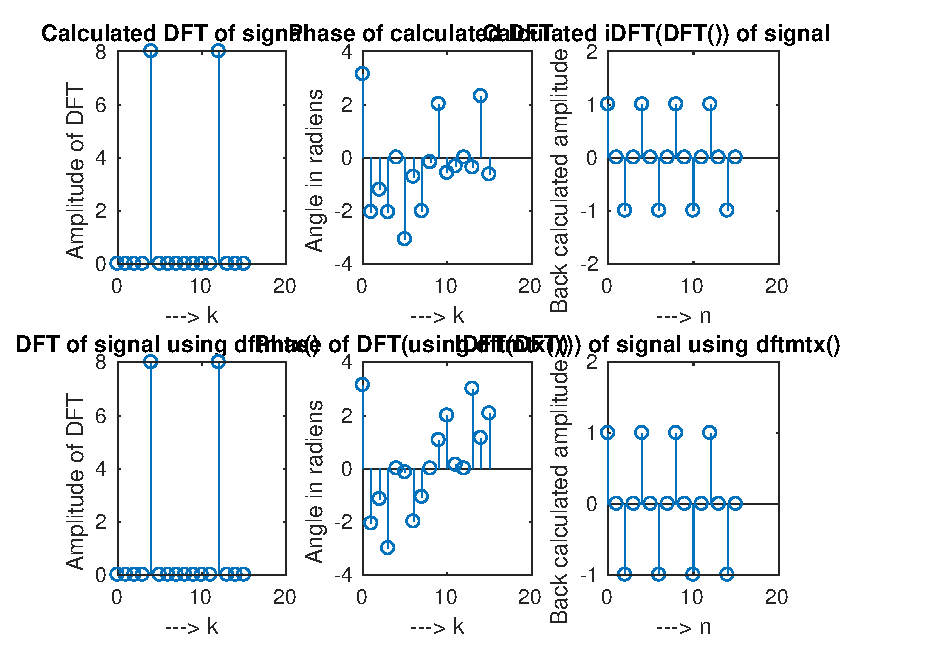
\includegraphics [width=4in]{L4Q3_02.eps}



\end{document}
    
